\documentclass[a4paper,showframe,11pt]{report}\usepackage[]{graphicx}\usepackage[]{color}
%% maxwidth is the original width if it is less than linewidth
%% otherwise use linewidth (to make sure the graphics do not exceed the margin)
\makeatletter
\def\maxwidth{ %
  \ifdim\Gin@nat@width>\linewidth
    \linewidth
  \else
    \Gin@nat@width
  \fi
}
\makeatother

\definecolor{fgcolor}{rgb}{0.196, 0.196, 0.196}
\newcommand{\hlnum}[1]{\textcolor[rgb]{0.063,0.58,0.627}{#1}}%
\newcommand{\hlstr}[1]{\textcolor[rgb]{0.063,0.58,0.627}{#1}}%
\newcommand{\hlcom}[1]{\textcolor[rgb]{0.588,0.588,0.588}{#1}}%
\newcommand{\hlopt}[1]{\textcolor[rgb]{0.196,0.196,0.196}{#1}}%
\newcommand{\hlstd}[1]{\textcolor[rgb]{0.196,0.196,0.196}{#1}}%
\newcommand{\hlkwa}[1]{\textcolor[rgb]{0.231,0.416,0.784}{#1}}%
\newcommand{\hlkwb}[1]{\textcolor[rgb]{0.627,0,0.314}{#1}}%
\newcommand{\hlkwc}[1]{\textcolor[rgb]{0,0.631,0.314}{#1}}%
\newcommand{\hlkwd}[1]{\textcolor[rgb]{0.78,0.227,0.412}{#1}}%
\let\hlipl\hlkwb

\usepackage{framed}
\makeatletter
\newenvironment{kframe}{%
 \def\at@end@of@kframe{}%
 \ifinner\ifhmode%
  \def\at@end@of@kframe{\end{minipage}}%
  \begin{minipage}{\columnwidth}%
 \fi\fi%
 \def\FrameCommand##1{\hskip\@totalleftmargin \hskip-\fboxsep
 \colorbox{shadecolor}{##1}\hskip-\fboxsep
     % There is no \\@totalrightmargin, so:
     \hskip-\linewidth \hskip-\@totalleftmargin \hskip\columnwidth}%
 \MakeFramed {\advance\hsize-\width
   \@totalleftmargin\z@ \linewidth\hsize
   \@setminipage}}%
 {\par\unskip\endMakeFramed%
 \at@end@of@kframe}
\makeatother

\definecolor{shadecolor}{rgb}{.97, .97, .97}
\definecolor{messagecolor}{rgb}{0, 0, 0}
\definecolor{warningcolor}{rgb}{1, 0, 1}
\definecolor{errorcolor}{rgb}{1, 0, 0}
\newenvironment{knitrout}{}{} % an empty environment to be redefined in TeX

\usepackage{alltt}
\usepackage{standalone}
\standalonetrue
\ifstandalone
  \usepackage{../../haziq_thesis}
  \usepackage{../../haziq_maths}
  \usepackage{../../haziq_glossary}
  \addbibresource{../../bib/haziq.bib}
  \externaldocument{../01/.texpadtmp/introduction}
\fi




\IfFileExists{upquote.sty}{\usepackage{upquote}}{}
\begin{document}

We illustrate the prediction of a real valued response when one of the covariates is a function using a widely analysed data set for quality control in the food industry. The data\footnotemark contain samples of spectrometric curve of absorbances of 215 pieces of finely chopped meat, along with their water, fat and protein content. These data are recorded on a Tecator Infratec Food and Feed Analyzer working in the wavelength range 850 - 1050 nm by the Near Infrared Transmission (NIT) principle. Absorption data has not been measured continuously, but instead 100 distinct wavelengths were obtained. Figure \ref{fig:tecator_data} shows a sample of 10 such spectrometric curves.

\footnotetext{Used with permission from Tecator (see \url{http://lib.stat.cmu.edu/datasets/tecator} for details). We used the version made available in the dataframe \code{tecator} from the \proglang{R} package \pkg{caret} for our analyses.}

\begin{knitrout}
\definecolor{shadecolor}{rgb}{1, 1, 1}\color{fgcolor}\begin{figure}[h]

{\centering 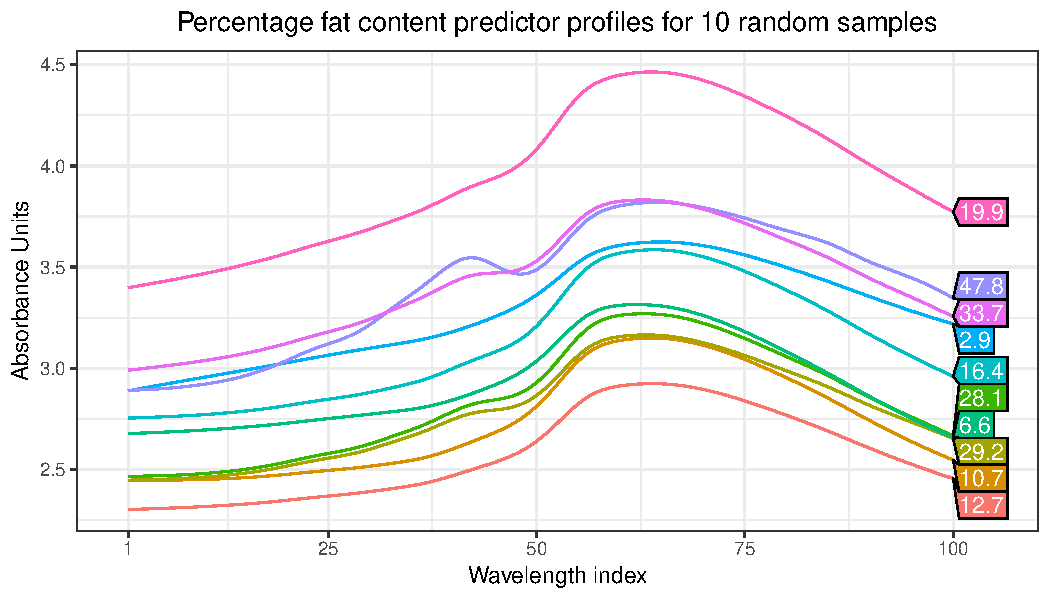
\includegraphics[width=0.9\linewidth]{figure/tecator_data-1} 

}

\caption[Sample of spectrometric curves used to predict fat content of meat]{Sample of spectrometric curves used to predict fat content of meat. For each meat sample the data consists of a 100 channel spectrum of absorbances and the contents of moisture, fat (numbers shown in boxes) and protein measured in percent. The absorbance is $- \log 10$ of the transmittance measured by the spectrometer. The three contents, measured in percent, are determined by analytic chemistry.}\label{fig:tecator_data}
\end{figure}


\end{knitrout}

For our analyses and many others' in the literature, the first 160 observations in the data set are used as a training sample for model fitting, and the remaining 55 observations as a test sample to evaluate the predictive performance of the fitted model. A summary of the various statistical methods applied to this data set, including various I-prior models, can be found in cite{bergsma2016}. The focus here is to use the \pkg{iprior} package to fit various I-prior models to the Tecator data set.

\hltodo[Necessary for functional covariates - approximation of the Sobolev-Hilbert space inner product]{Before we began, we preprocessed the spectral curves by taking their first differences}. This leaves us with the 99-dimensional covariate, which is saved in the matrix object named \code{absorpTrain}. Our first modelling attempt is to estimate a linear effect by regressing the responses \code{fatTrain} against only a single high-dimensional covariate \code{absorpTrain} using the canonical RKHS. The model is loaded as an \code{ipriorKernel} object as follows:

\begin{knitrout}
\definecolor{shadecolor}{rgb}{1, 1, 1}\color{fgcolor}\begin{kframe}
\begin{alltt}
\hlstd{R> }\hlcom{# Model 1: canonical RKHS (linear)}
\hlstd{R> }\hlstd{(mod1} \hlkwb{<-} \hlkwd{kernL}\hlstd{(}\hlkwc{y} \hlstd{= fatTrain, absorpTrain))}
\end{alltt}
\begin{verbatim}
## 
## Sample size =  160 
## Number of x variables, p =  1 
## Number of scale parameters, l =  1 
## Number of interactions =  0 
## 
## Info on H matrix:
## 
## List of 1
##  $ absorpTrain: Canonical [1:160, 1:160] 0.000254 0.0003 -0.000231 -..
\end{verbatim}
\end{kframe}
\end{knitrout}

Here, we have used the non-formula syntax because each object after the \code{y} argument is treated as a single covariate, even if it is multi-dimensional, i.e., a matrix. We could have also used the formula syntax and used the \code{model} option \code{one.lam = TRUE}. Note that the canonical RKHS is used by default.

Our second and third model uses a polynomial-type construction of the canonical RKHS, which allows us to add quadratic and cubic terms of the spectral curves. The syntax is as before with the addition of \verb@absorpTrain^b@, which element-wise raises the entries of the matrix  \code{absorpTrain} to the power \code{b}. To date, the only method to fit these models parsimoniously in \pkg{iprior} is by using non-formula syntax with \code{model} option \code{order} to control the scale parameters of the RKHS. Both models only have a single parameter. Without specifying the \code{order} option, additional scale parameters would be fitted, one for each quadratic and cubic term.

\begin{knitrout}
\definecolor{shadecolor}{rgb}{1, 1, 1}\color{fgcolor}\begin{kframe}
\begin{alltt}
\hlstd{R> }\hlcom{# Model 2: canonical RKHS (quadratic)}
\hlstd{R> }\hlstd{mod2} \hlkwb{<-} \hlkwd{kernL}\hlstd{(}\hlkwc{y} \hlstd{= fatTrain, absorpTrain, absorpTrain} \hlopt{^} \hlnum{2}\hlstd{,}
\hlstd{+  }              \hlkwc{model} \hlstd{=} \hlkwd{list}\hlstd{(}\hlkwc{order} \hlstd{=} \hlkwd{c}\hlstd{(}\hlstr{"1"}\hlstd{,} \hlstr{"1^2"}\hlstd{)))}
\end{alltt}
\end{kframe}
\end{knitrout}
\begin{knitrout}
\definecolor{shadecolor}{rgb}{1, 1, 1}\color{fgcolor}\begin{kframe}
\begin{alltt}
\hlstd{R> }\hlcom{# Model 3: canonical RKHS (cubic)}
\hlstd{R> }\hlstd{mod3} \hlkwb{<-} \hlkwd{kernL}\hlstd{(}\hlkwc{y} \hlstd{= fatTrain, absorpTrain, absorpTrain} \hlopt{^} \hlnum{2}\hlstd{, absorpTrain} \hlopt{^} \hlnum{3}\hlstd{,}
\hlstd{+  }              \hlkwc{model} \hlstd{=} \hlkwd{list}\hlstd{(}\hlkwc{order} \hlstd{=} \hlkwd{c}\hlstd{(}\hlstr{"1"}\hlstd{,} \hlstr{"1^2"}\hlstd{,} \hlstr{"1^3"}\hlstd{)))}
\end{alltt}
\end{kframe}
\end{knitrout}

Next, we fitted a smooth dependence of fat content on the spectrometric curves using the FBM RKHS. By default, the Hurst coefficient for the FBM RKHS is set to be 0.5. However, we can use the function \code{fbmOptim()} which is able to compute the maximum likelihood estimate for the Hurst coefficient.

\begin{knitrout}
\definecolor{shadecolor}{rgb}{1, 1, 1}\color{fgcolor}\begin{kframe}
\begin{alltt}
\hlstd{R> }\hlcom{# Model 4: FBM RKHS (default Hurst = 0.5)}
\hlstd{R> }\hlstd{mod4} \hlkwb{<-} \hlkwd{kernL}\hlstd{(}\hlkwc{y} \hlstd{= fatTrain, absorpTrain,} \hlkwc{model} \hlstd{=} \hlkwd{list}\hlstd{(}\hlkwc{kernel} \hlstd{=} \hlstr{"FBM"}\hlstd{))}
\end{alltt}
\end{kframe}
\end{knitrout}
\begin{knitrout}
\definecolor{shadecolor}{rgb}{1, 1, 1}\color{fgcolor}\begin{kframe}
\begin{alltt}
\hlstd{R> }\hlstd{mod4}
\end{alltt}
\begin{verbatim}
## 
## Sample size =  160 
## Number of x variables, p =  1 
## Number of scale parameters, l =  1 
## Number of interactions =  0 
## 
## Info on H matrix:
## 
## List of 1
##  $ absorpTrain: FBM,0.5 [1:160, 1:160] 0.016192 -0.000775 -0.00346 -..
\end{verbatim}
\end{kframe}
\end{knitrout}
Finally, we add an extra covariate (meat moisture content) which is assumed to have a linear effect on fat content. Doing so adds one extra parameter to the model. To specify multiple kernels, we need to include the \code{model} option \code{kernel = c("FBM", "Canonical")} to indicate the effect of the respective covariates on the response. This is verified by inspecting the \code{print} output of the \code{ipriorKernel} object, and indeed we see that there are now two scale parameters, and the kernel loader correctly assigns the FBM and canonical RKHS to the spectrometric curves and moisture content respectively.

\begin{knitrout}
\definecolor{shadecolor}{rgb}{1, 1, 1}\color{fgcolor}\begin{kframe}
\begin{alltt}
\hlstd{R> }\hlcom{# Model 5: FBM RKHS + extra covariate}
\hlstd{R> }\hlstd{(mod5} \hlkwb{<-} \hlkwd{kernL}\hlstd{(}\hlkwc{y} \hlstd{= fatTrain, absorpTrain, waterTrain,}
\hlstd{+  }               \hlkwc{model} \hlstd{=} \hlkwd{list}\hlstd{(}\hlkwc{kernel} \hlstd{=} \hlkwd{c}\hlstd{(}\hlstr{"FBM"}\hlstd{,} \hlstr{"Canonical"}\hlstd{))))}
\end{alltt}
\begin{verbatim}
## 
## Sample size =  160 
## Number of x variables, p =  2 
## Number of scale parameters, l =  2 
## Number of interactions =  0 
## 
## Info on H matrix:
## 
## List of 2
##  $ absorpTrain: FBM,0.5 [1:160, 1:160] 0.016192 -0.000775 -0.00346 -..
##  $ waterTrain : Canonical [1:160, 1:160] 10.9 58.9 -23.8 -29.7 18.2 ..
\end{verbatim}
\end{kframe}
\end{knitrout}


All of the above models were fitted using \code{ipriorOptim}, except for the last two model, where we used \code{fbmOptim} in order to obtain the maximum likelihood estimate for the Hurst coefficient of the FBM RKHS. Predicted values of the test data set can be obtained using the \code{predict} function

\begin{knitrout}
\definecolor{shadecolor}{rgb}{1, 1, 1}\color{fgcolor}\begin{kframe}
\begin{alltt}
\hlstd{R> }\hlstd{fatTestPredicted} \hlkwb{<-} \hlkwd{predict}\hlstd{(mod1.fit,} \hlkwd{list}\hlstd{(absorpTest))}
\hlstd{R> }\hlkwd{head}\hlstd{(fatTestPredicted)}
\end{alltt}
\begin{verbatim}
## [1] 14.12268 15.85864 15.84706 21.59324 25.22315 26.57978
\end{verbatim}
\end{kframe}
\end{knitrout}

and the root mean squared error (RMSE) calculated for each of the models. It was noted that for some models, different EM starting values gave slightly different results, and we suspect this is a due to numerical issues with the computation of the variance of marginal I-prior distribution. Nonetheless, the predicted values, and hence the RMSE, remain fairly robust.

The results are summarised in Table \ref{tab:tecator}. Models 1-3 have the same number of parameters, so a direct comparison can be done, with the model giving the highest likelihood value preferred. In this case, it is the model with a quadratic effect, giving a test RMSE of 1.23. Models with the FBM RKHS gave better prediction still. A smooth effect (Hurst = 0.5) yields a test RMSE of 0.67, and this is improved only slightly by using the maximum likelihood estimate for the Hurst coefficient of 0.519. The best predictive model obtained was the final model, i.e., a smooth effect (Hurst = 0.934) with an additional covariate, giving a test RMSE of 0.68.

\newcolumntype{R}[1]{>{\raggedleft\arraybackslash}p{#1}}
\begin{table}[ht]
\centering
\begin{tabular}{ll R{1.7cm} rr}
\toprule
&&{{Log-}}&\multicolumn{2}{c}{RMSE} \\
\cline{4-5}
Model
&I-prior effect
&{likelihood}
&{\small Train}
&{\small Test} \\
\midrule
1     & Linear
& $-$409.32
& 2.85
& 3.24 \\
2     & Quadratic
& $-$279.64
& 0.72
& 1.23 \\
3     & Cubic
& $-$301.26
& 0.99
& 1.65 \\
4     & Smooth (Hurst = 0.5)
& $-$148.34
& 0.00
& 0.67 \\
4a     & Smooth (Hurst = 0.519)
& $-$146.23
& 0.00
& 0.66 \\
5     & Smooth (Hurst = 0.934) with additional covariate
& $-$213.51
& 0.31
& 0.54 \\
\bottomrule
\end{tabular}
\caption{A summary of the I-prior models fitted on the Tecator data set.}
\label{tab:tecator}
\end{table}

\end{document}


